%% abtex2-modelo-slides.tex, v-1.0 gfabinhomat
%% Copyright 2012-<COPYRIGHT_YEAR> by abnTeX2 group at http://www.abntex.net.br/ 
%%
%% This work may be distributed and/or modified under the
%% conditions of the LaTeX Project Public License, either version 1.3
%% of this license or (at your option) any later version.
%% The latest version of this license is in
%%   http://www.latex-project.org/lppl.txt
%% and version 1.3 or later is part of all distributions of LaTeX
%% version 2005/12/01 or later.
%%
%% This work has the LPPL maintenance status `maintained'.
%% 
%% The Current Maintainer of this work is Fábio Rodrigues Silva, 
%% member of abnTeX2 team, led by Lauro César Araujo. 
%% Further information are available on 
%% http://www.abntex.net.br/
%%
%% This work consists of the files abntex2-modelo-slides.tex, 
%% abntex2-modelo-references.bib and abntex2-modelo-marca.pdf
%%
%% Modelo desenvolvido por Fábio Rodrigues Silva (gfabinhomat@gmail.com)
%% Mais informações podem ser obtidas no guia do usuário Beamer 
%% (http://linorg.usp.br/CTAN/macros/latex/contrib/beamer/doc/beameruserguide.pdf)
%% Informações rápidas podem ser acessadas em http://en.wikibooks.org/wiki/LaTeX/Presentations

\pdfminorversion=7

% Apresentações em widescreen. Outros valores possíveis: 1610, 149, 54, 43 e 32.
% Por padrão, as apresentações são no formato 4:3 (sem o aspectratio).
    \documentclass[aspectratio=43]{beamer}	 	

\usetheme{PaloAlto}
\usecolortheme{spruce}
% Enconte mais temas e cores em http://www.hartwork.org/beamer-theme-matrix/ 
% Veja também http://deic.uab.es/~iblanes/beamer_gallery/index.html

\definecolor{ifprgreen}{RGB}{0,61,30}
\definecolor{ifprlightgreen}{RGB}{139,239,67}
\definecolor{ifprred}{RGB}{212,0,0}

% Customizações de Cores: fg significa cor do texto e bg é cor do fundo
%\setbeamercolor{normal text}{fg=black}
%\setbeamercolor{alerted text}{fg=red}
%\setbeamercolor{frametitle}{fg=black}
%\setbeamercolor{framesubtitle}{fg=black}
\setbeamercolor{block title}{bg=ifprgreen}		%Cor do título
%\setbeamercolor{block body}{bg=lightgray, fg=darkgray}	%Cor do texto (bg= fundo; fg=texto)
%\setbeamercolor{section in sidebar}{bg=ifprlightgreen, fg=black}
\setbeamercolor{itemize item}{fg=yellow,bg=black}
\setbeamercolor*{item}{fg=ifprgreen}
\setbeamercolor{section in toc}{fg=black}
\setbeamercolor{caption name}{fg=black}

\setbeamertemplate{caption}[numbered]

\makeatletter
\logo{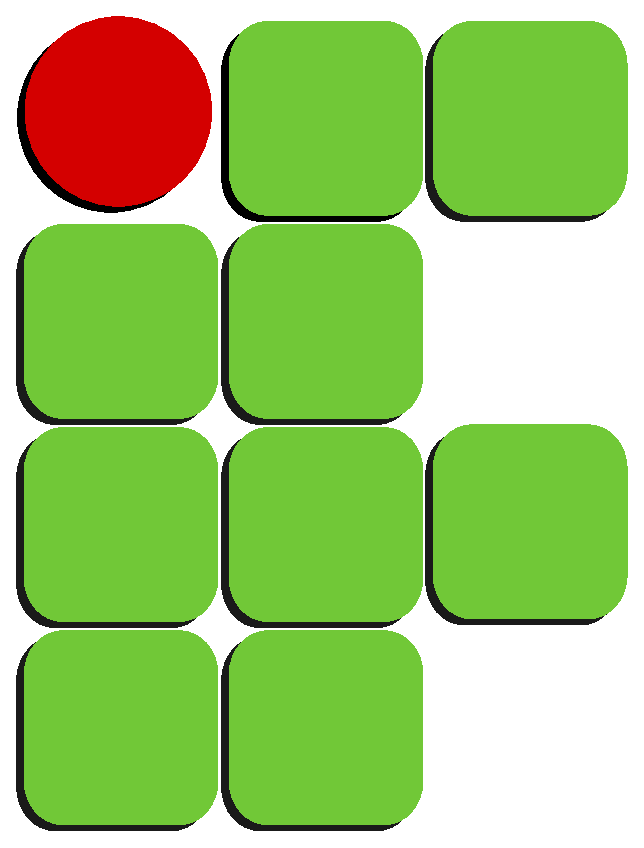
\includegraphics[height=.9\beamer@headheight]{logo_ifpr_shadow.eps}}
\makeatother

\makeatletter
  \setbeamertemplate{sidebar \beamer@sidebarside}
  {
    \beamer@tempdim=\beamer@sidebarwidth%
    \advance\beamer@tempdim by -6pt%
    \vskip4em%
    \insertverticalnavigation{\beamer@sidebarwidth}%
    \vfill
    \ifx\beamer@sidebarside\beamer@lefttext%
    \else%
      \usebeamercolor{normal text}%
      \llap{\usebeamertemplate***{navigation symbols}\hskip0.1cm}%
      \vskip2pt%
    \fi%
  }%

  \ifx\beamer@sidebarside\beamer@lefttext%
    \defbeamertemplate*{sidebar right}{sidebar theme}
    {%
      \vfill%
      \llap{\usebeamertemplate***{navigation symbols}\hskip0.1cm}%
      \vskip2pt}
  \fi
\makeatother

% ---
% PACOTES
% ---
\usepackage[alf]{abntex2cite}		% Citações padrão ABNT
\usepackage[brazil]{babel}		% Idioma do documento
\usepackage{color}			% Controle das cores
\usepackage{xcolor}			% Controle das cores
\usepackage[T1]{fontenc}		% Selecao de codigos de fonte.
\usepackage{graphicx}			% Inclusão de gráficos
\usepackage[utf8]{inputenc}		% Codificacao do documento (conversão automática dos acentos)
\usepackage{txfonts}			% Fontes virtuais
\usepackage{graphbox}
\usepackage{pgf}  
\usepackage{tikz}
\usepackage[default]{lato}
\usepackage{tabularx}
% ---

% --- Informações do documento ---
\title{Automatização de Mineração de criptomoedas Com Distribuição Linux}
\author{Mateus Bittencourt Mercer \\ Prof\@. Dr\@. Rodolfo Barriviera}
\institute{Instituto Federal do Paraná Campus Londrina}
\date{\today}
% ---

% ---
% Caminho das imagens
% ---
\graphicspath{{imagens/}}

% ----------------- INÍCIO DO DOCUMENTO --------------------------------------
\begin{document}

% ----------------- NOVO SLIDE --------------------------------
\begin{frame}
\titlepage
\end{frame}

% ----------------- NOVO SLIDE --------------------------------
\begin{frame}{Sumário}
\tableofcontents
\end{frame}

% ----------------- NOVO SLIDE --------------------------------
\section{Objetivos}

\begin{frame}{Objetivo Geral}

\noindent\makebox[\textwidth][c]{%
\begin{minipage}{10cm}
    Utilizar uma distribuição Linux para automatizar a configuração
    do software de criptomoeda para otimizar o tempo de instalação do
    usuário.
\end{minipage}
}

\end{frame}

% ----------------- NOVO SLIDE --------------------------------
\begin{frame}{Objetivos Específicos}

\begin{itemize} 

    \item Buscar alternativas de personalização de uma distribuição
        Linux para a automatização da instalação dos drivers
        genéricos;

    \item Pesquisar diferentes criptomoedas e suas vantagens e
        desvantagens em diferentes hardwares;

    \item Encontrar as melhores alternativas de softwares em termos de
        praticidade e tempo;

    \item Comparar distribuições para a customização;

    \item Customizar uma distribuição;

    \item Fazer um comparativo da velocidade de instalação entre a
distribuição e uma instalação manual.

\end{itemize}
\end{frame}

% ----------------- NOVO SLIDE --------------------------------
\section{Introdução}
\begin{frame}
\frametitle{Introdução}
\framesubtitle{Definição e Contexto das Criptomoedas}

%\begin{block}{Título}
% Este modelo foi preparado como uma aplicação do uso do pacote abnTeX2 com o Beamer.
%\end{block}
\begin{itemize}
    \item Criptomoedas são um sistema descentralizado
        \cite{Prado2017}
    
    \item A maioria implementa a transferência de \emph{tokens}

    \item A validação destas transferências é feita por propriedades
        matemáticas \cite{LChicarino}

    \item Esta validação é independente de uma instituição financeira
        \cite{Nakamoto2008}

    \item O Bitcoin é a criptomoeda mais utilizada atualmente

    \item Criptomoedas que surgiram após o Bitcoin são denominadas
        \emph{alt coins}
\end{itemize}



\begin{block}{Curiosidade}
    Existem mais de $800$ \emph{alt coins} registradas no site Coin
    Market Cap \cite{Arsov, CoinMarketCap2018}.
\end{block}

\end{frame}

% ----------------- NOVO SLIDE --------------------------------
\begin{frame}
    \frametitle{Introdução}
    \framesubtitle{Mineração e as Dificuldades na sua Configuração}
    
    \begin{itemize}
        \item Minerar uma criptomoeda que usa uma tecnologia de blockchain
            nada mais é que continuar as transações

        \item Quem minera recebe $N$ tokens por $N$ trabalho
            feito

        \item Por existir uma variedade de criptomoedas e hardwares,
            suas implementações variam

        \item Configurar uma distribuição Linux para fazer a mineração
            de uma criptomoeda requer tempo e um conhecimento técnico
            moderado
        
        \item Nem sempre a mineração é lucrativa
    \end{itemize}
\end{frame}

% ----------------- NOVO SLIDE --------------------------------
\section[Desenvolvi\ldots]{Desenvolvimento}

\begin{frame}
    \frametitle{Desenvolvimento}
    \framesubtitle{O Bitcoin e o Blockchain}
    
    \begin{itemize}
        \item Em vez de existir um balanço em uma conta, existe uma lista de
            transações feitas desde o início do sistema
            \cite{Weber2012}

        \item O Blockchain se a assemelha a um histórico em formato de
            lista encadeada

        \item Cada parte deste bloco (conjunto de transações) deve ser
            validado, esse processo é chamado de mineração
            \cite{LChicarino}

        \item Usuários são identificados por uma chave pública e
            acessam sua carteira com uma chave privada
        
    \end{itemize}
\end{frame}

% ----------------- NOVO SLIDE --------------------------------
\begin{frame}
    \frametitle{Desenvolvimento}
    \framesubtitle{Transação de Bitcoin Resumida}
    
    \begin{figure}[H]
        \caption{\label{fig:exemplo-bitcoin}Exemplo de uma transferência
            com Bitcoin.}
        \begin{center}
            \includegraphics[width=.6\linewidth]{exemplo-bitcoin.pdf}
        \end{center}
        Fonte: O Autor.
    \end{figure}
\end{frame}

% ----------------- NOVO SLIDE --------------------------------
\begin{frame}
    \frametitle{Desenvolvimento}
    \framesubtitle{Ethereum e Contratos Inteligentes}
    
    \begin{itemize}
        \item O Ethereum foca na implementação de uma linguagem de
            programação Turing completa para a criação de scripts ou
            ``contratos inteligentes'' \cite{Narayanan2016}

        \item Contratos inteligentes são programas que podem ser
            executados no Blockchain
    \end{itemize}

    \begin{block}{Segurança}
        As criptomoedas permitem a transferência de tokens de maneira
        extremamente segura. Contratos inteligentes permitem que
        qualquer aplicação possa ser implementada com o proveito dessa
        segurança.
    \end{block}
\end{frame}

% ----------------- NOVO SLIDE --------------------------------
\begin{frame}
    \frametitle{Desenvolvimento}
    \framesubtitle{Exemplo de Contrato Inteligente em Ethereum}
\begin{figure}[H]
    \caption{\label{fig:contratos-inteligentes}Exemplo de um contrato
    inteligente em Ethereum.}
    \begin{center}
        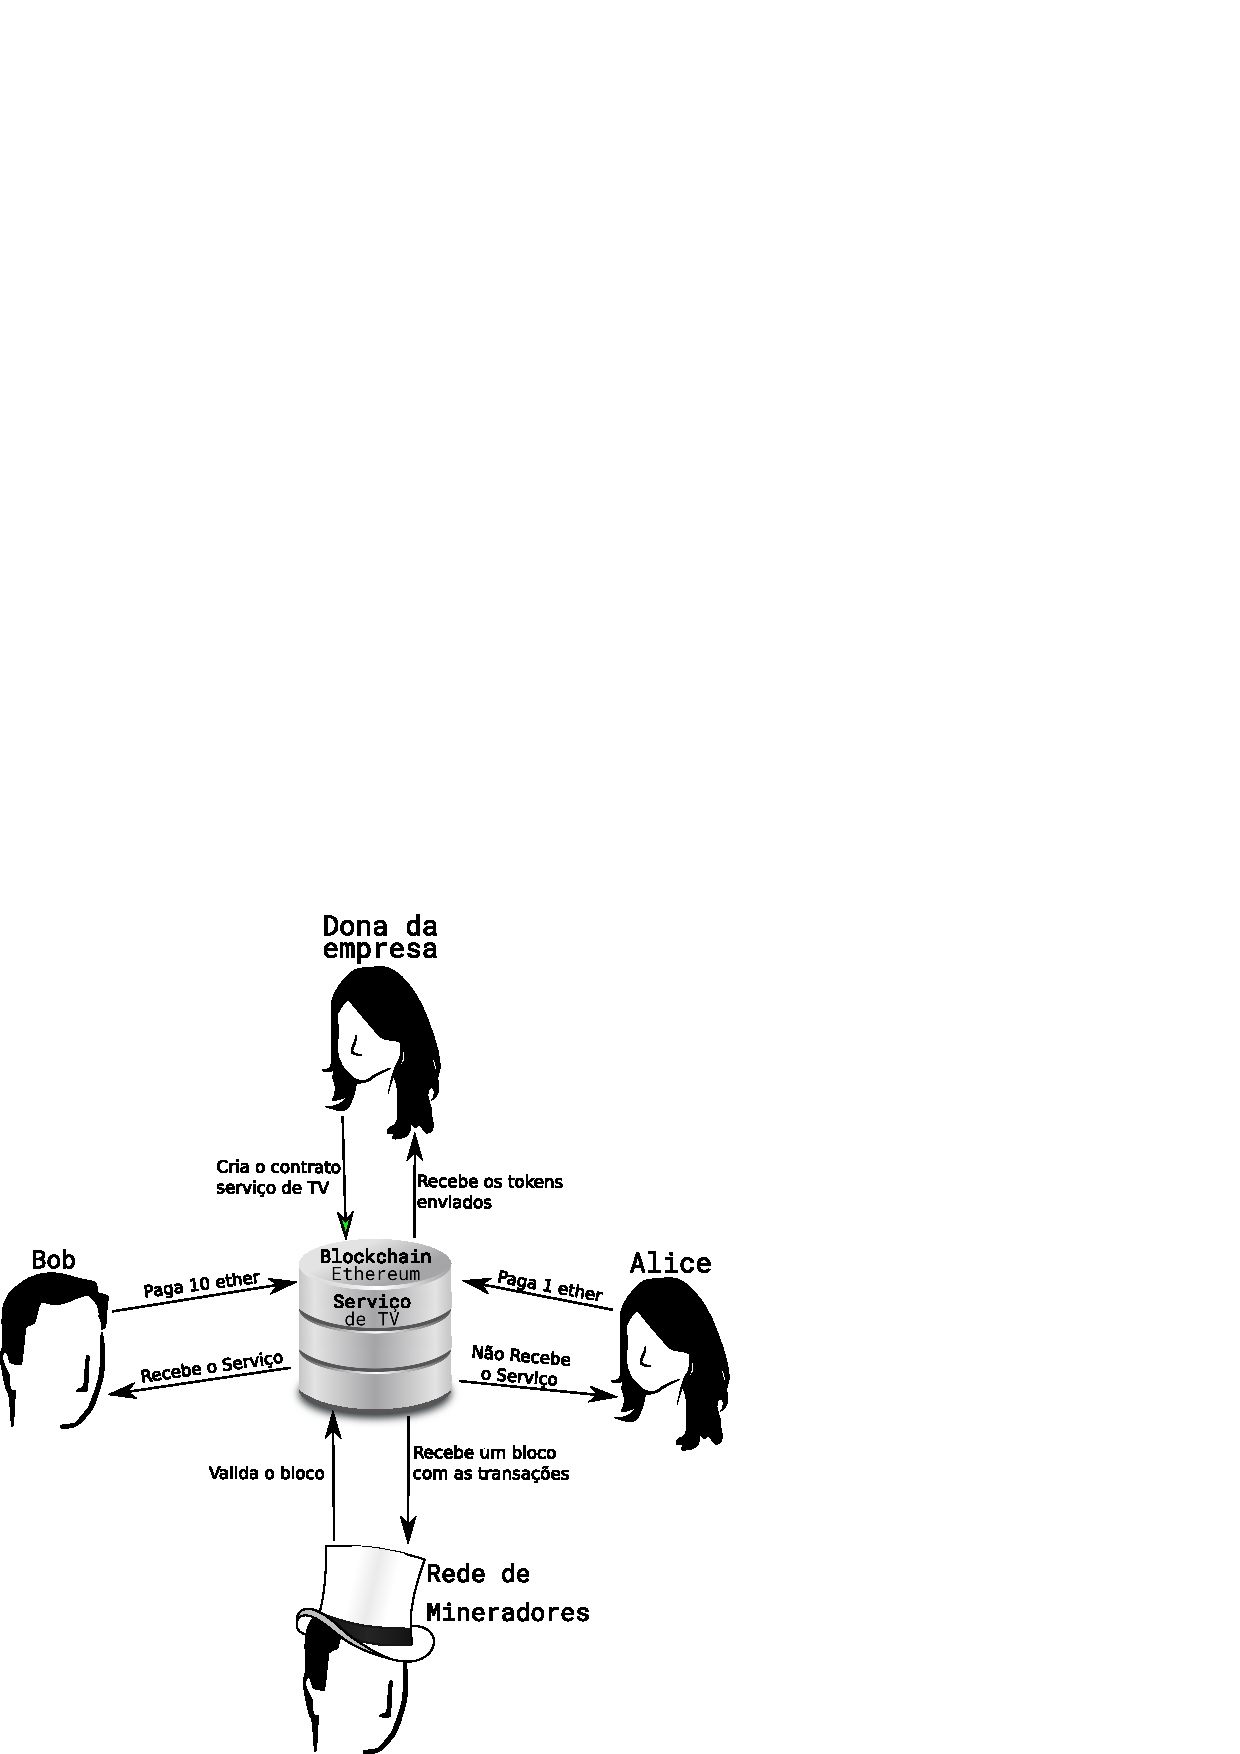
\includegraphics[width=.5\linewidth]{contratos-inteligentes.pdf}
    \end{center}
    Fonte: O Autor.
\end{figure}

\end{frame}

% ----------------- NOVO SLIDE --------------------------------
\begin{frame}
    \frametitle{Desenvolvimento}
    \framesubtitle{Mineração}

    \begin{itemize}
        \item O incentivo da mineração é a recompensa
            \cite{LChicarino}

        \item A prova de trabalho existe para evitar que uma transação
            aconteça duas vezes

        \item Próximos blocos do blockchain são sempre baseados em
            blocos anteriores \cite{Nakamoto2008, Dev2014}
        
        \item A variedade de algoritmos de mineração permite que
            alguns chips ASIC's sejam criados \cite{Smith1997}

        \item Algumas criptomoedas implementam algoritmos que
            dificultam a criação de ASIC's \cite{NiceHash2018}

    \end{itemize}
\end{frame}

% ----------------- NOVO SLIDE --------------------------------
\begin{frame}
    \frametitle{Desenvolvimento}
    \framesubtitle{Rigs de Mineração}

    \begin{itemize}
        \item Quanto mais poder computacional, mais lucrativa é a
            mineração (o algoritmo interfere diretamente)

        \item A maioria das criptomoedas permitem a mineração por uma
            placa gráfica

        \item Um rig de mineração é um sistema computacional que tem
            como responsabilidade a mineração de uma criptomoeda
            \cite{BitcoinWiki2015}

        \item A medida utilizada para apresentar o desempenho de um
            rig de mineração é ``hashes por segundo'' $h/s$

    \end{itemize}
\end{frame}

% ----------------- NOVO SLIDE --------------------------------
\begin{frame}
    \frametitle{Desenvolvimento}
    \framesubtitle{Rigs de Mineração}

    \begin{figure}[H]
        \caption{\label{fig:rig_mineracao}Um rig de mineração com 13 GPUs
        NVidia 1060}
        \begin{center}
            \includegraphics[width=.3\linewidth]{rig_mineracao.png}
        \end{center}
        \legend{Fonte: \url{https://mining.bg/13-gpu-mining-rig-nvidia-1060-3gb-8/}}
    \end{figure}
\end{frame}

% ----------------- NOVO SLIDE --------------------------------
\begin{frame}
    \frametitle{Desenvolvimento}
    \framesubtitle{Distribuições Linux}

    \begin{itemize}
        \item Assim como as criptomoedas, a variedade de distribuições
            é extensa

        \item Distribuição Linux é uma variação do sistema operacional
            Linux para um determinado contexto

        \item Uma distribuição Linux pode ser baseada em outra

    \end{itemize}
\end{frame}

% ----------------- NOVO SLIDE --------------------------------
\begin{frame}
    \frametitle{Desenvolvimento}
    \framesubtitle{Customização de Distribuições Linux}

    \begin{itemize}
        \item Essa customização pode ser feita de duas maneiras

        \item Criação com o código fonte ou modificação da existente

        \item A criação com código fonte exige um conhecimento maior
            em programação de baixo nível

        \item Existem ferramentas gráficas para a criação de
            distribuições Linux, como o Respin \cite{Respin2018}

    \end{itemize}
\end{frame}

% ----------------- NOVO SLIDE --------------------------------
\section{Metodologia}

% ----------------- NOVO SLIDE --------------------------------
\section{Resultados Parciais}

% ----------------- NOVO SLIDE --------------------------------
\section{Considerações Finais}

% ----------------- NOVO SLIDE --------------------------------

% \section{Referências}

% --- O comando \allowframebreaks ---
% Se o conteúdo não se encaixa em um quadro, a opção allowframebreaks instrui 
% beamer para quebrá-lo automaticamente entre dois ou mais quadros,
% mantendo o frametitle do primeiro quadro (dado como argumento) e acrescentando 
% um número romano ou algo parecido na continuação.

\begin{frame}<presentation:0>[noframenumbering]
\bibliography{referencias}
\end{frame}

% ----------------- FIM DO DOCUMENTO -----------------------------------------
\end{document}
